\chapter{Les glucides}\label{ch:b1:carbohydrates}

Une pomme de terre et une \omterm{def:b1:flowering-plant-organization:organs}{feuille} de papier sont faites de la même
molécule, le glucose, enfilé en chaînes. L'une est un repas et l'autre
non, parce que les chaînes sont unies par deux liaisons différentes~: la
liaison $\alpha$ de l'\omterm{def:b1:carbohydrates:polysaccharide}{amidon} enroule la chaîne en une hélice que nos
enzymes ouvrent, la liaison $\beta$ de la \omterm{def:b1:carbohydrates:polysaccharide}{cellulose} l'étire en rubans
qui s'empilent en fibres qu'aucun mammifère ne digère. Un foie stocke
cent grammes de glucose sous forme de \omterm{def:b1:carbohydrates:polysaccharide}{glycogène}, un arbre se tient
debout grâce à la \omterm{def:b1:carbohydrates:polysaccharide}{cellulose}, un scarabée porte de la \omterm{def:b1:carbohydrates:polysaccharide}{chitine}, et chaque
\omterm{def:b1:cell-unit-of-life:cell}{cellule} expose des sucres à sa surface comme identité. Ce chapitre
décrit les sucres simples, les liaisons qui les unissent, les
\omterm{def:b1:carbohydrates:polysaccharide}{polysaccharides} qu'ils bâtissent, et les molécules décorées de sucres de
la surface cellulaire et de la paroi végétale.

\section{Les monosaccharides}

\begin{definition}[Monosaccharide]\label{def:b1:carbohydrates:monosaccharide}
Les \emph{glucides}\index{glucide} sont les molécules de composition
$(\mathrm{CH_2O})_n$ et leurs dérivés. Un
\emph{monosaccharide}\index{monosaccharide} (sucre simple, ou ose) est
une chaîne de trois à sept carbones, dont l'un porte un groupe carbonyle
et les autres des hydroxyles~: c'est un \emph{aldose}\index{aldose}
quand le carbonyle est terminal (un aldéhyde~: glucose, galactose,
ribose), un \emph{cétose}\index{cetose@cétose} quand il est interne (une
cétone~: fructose). Par la longueur~: trioses ($n = 3$~:
glycéraldéhyde), pentoses ($n = 5$~: ribose, désoxyribose), hexoses
($n = 6$~: glucose, fructose, galactose). Tout carbone portant quatre
groupes différents est un centre \emph{chiral}, de sorte que chaque
formule recouvre plusieurs \emph{stéréo-isomères}~: le glucose a quatre
carbones chiraux et seize isomères, dont les êtres vivants n'emploient
qu'un seul, le D-glucose. Les \emph{épimères} ne diffèrent que par un
carbone (le glucose et le galactose en C4).
\end{definition}

\begin{proposition}[Formes cycliques et anomères]\label{prop:b1:carbohydrates:rings}
\index{anomere@anomère}\index{projection de Haworth}
Dans l'eau, un pentose ou un hexose est presque entièrement cyclisé~: le
carbone du carbonyle réagit avec un hydroxyle de la même molécule (C5
chez le glucose) pour fermer un cycle \emph{pyranose} à six sommets ou
un cycle \emph{furanose} à cinq (fructose, ribose). Le carbone du
carbonyle devient un nouveau centre chiral, le \emph{carbone
anomérique}, dont l'hydroxyle peut se placer sous le plan du cycle
(anomère $\alpha$) ou au-dessus (anomère $\beta$) dans la représentation
de Haworth~; les deux formes s'interconvertissent en quelques minutes
par la chaîne ouverte. En solution, le glucose est à \qty{36}{\%}
$\alpha$, à \qty{64}{\%} $\beta$ et à moins de \qty{0.1}{\%} en chaîne
ouverte. C'est le carbone anomérique libre qui rend un sucre
\emph{réducteur}~: il peut s'ouvrir et réduire un réactif au cuivre ou à
l'argent.
\end{proposition}

\begin{omfigure}
\begin{tikzpicture}[font=\footnotesize, line cap=round, line join=round]
  \newcommand{\haworth}[2]{%
    % ring: C5 top-left, O top-right, C1 right, C2 bottom-right, C3 bottom-left, C4 left (scaled 1.4)
    \draw[thick] (0.84,1.54) -- (2.52,1.54) -- (3.64,0.42) -- (2.52,-0.7) -- (0.84,-0.7) -- (-0.28,0.42) -- cycle;
    \draw[line width=3.5pt] (0.84,-0.7) -- (2.52,-0.7);
    \draw[line width=2.5pt] (2.52,-0.7) -- (3.64,0.42);
    \draw[line width=2.5pt] (0.84,-0.7) -- (-0.28,0.42);
    \node[fill=white, inner sep=1pt] at (2.52,1.54) {O};
    \node[font=\scriptsize] at (3.25,0.42) {1};
    \node[font=\scriptsize] at (2.45,-0.35) {2};
    \node[font=\scriptsize] at (0.9,-0.35) {3};
    \node[font=\scriptsize] at (0.1,0.42) {4};
    \node[font=\scriptsize] at (0.95,1.2) {5};
    % C5: CH2OH up
    \draw (0.84,1.54) -- (0.84,2.2) node[above] {$\mathrm{CH_2OH}$};
    % C4: OH down, H up
    \draw (-0.28,0.42) -- (-0.28,1.05) node[above] {H};
    \draw (-0.28,0.42) -- (-0.28,-0.2) node[below] {OH};
    % C3: OH up
    \draw (0.84,-0.7) -- (0.84,-0.05) node[above, xshift=-3pt] {OH};
    \draw (0.84,-0.7) -- (0.84,-1.3) node[below] {H};
    % C2: OH down
    \draw (2.52,-0.7) -- (2.52,-1.3) node[below] {OH};
    \draw (2.52,-0.7) -- (2.52,-0.05) node[above, xshift=3pt] {H};
    % C1: anomeric
    \draw (3.64,0.42) -- (3.64,1.05) node[above] {#1};
    \draw (3.64,0.42) -- (3.64,-0.2) node[below] {#2};
  }
  \begin{scope}
    \haworth{H}{OH}
    \node[anchor=north, align=center] at (1.7,-1.9) {$\alpha$-D-glucose\\ OH anomérique (carbone 1) sous le cycle};
  \end{scope}
  \begin{scope}[xshift=8.4cm]
    \haworth{OH}{H}
    \node[anchor=north, align=center] at (1.7,-1.9) {$\beta$-D-glucose\\ OH anomérique (carbone 1) au-dessus du cycle};
  \end{scope}
  \draw[<->, thick, gray] (4.9,0.42) -- (7.4,0.42) node[midway, above, align=center] {chaîne ouverte\\ (aldéhyde)};
\end{tikzpicture}

{\small Les deux anomères du D-glucose en \omterm{prop:b1:carbohydrates:rings}{projection de Haworth}~: le
cycle vu par la tranche, son arête épaisse vers le lecteur, l'hydroxyle
du carbone anomérique 1 sous le plan ($\alpha$) ou au-dessus ($\beta$).
Ils s'interconvertissent par l'aldéhyde à chaîne ouverte.}
\end{omfigure}

\begin{method}[Lire une projection de Haworth]\label{met:b1:carbohydrates:haworth}
\begin{enumerate}
  \item Repérer l'oxygène du cycle~; le carbone anomérique (C1 dans un
        \omterm{def:b1:carbohydrates:monosaccharide}{aldose}, C2 dans un \omterm{def:b1:carbohydrates:monosaccharide}{cétose}) est le carbone du cycle situé à sa
        droite, portant à la fois un hydroxyle et l'oxygène du cycle.
  \item Le carbone portant le groupe $\mathrm{CH_2OH}$ à l'extérieur du
        cycle (C5 chez le glucose) est à gauche de l'oxygène du cycle~;
        son $\mathrm{CH_2OH}$ pointe vers le haut dans un sucre D.
  \item Hydroxyle anomérique vers le bas~: $\alpha$~; vers le haut (du
        même côté que $\mathrm{CH_2OH}$)~: $\beta$.
  \item Comparer les autres hydroxyles à ceux du glucose (bas, haut, bas
        pour C2, C3, C4)~: une seule différence identifie un épimère (le
        galactose~: C4 vers le haut).
\end{enumerate}
\end{method}

\begin{example}[Des sucres qui ne sont pas $(\mathrm{CH_2O})_n$]\label{ex:b1:carbohydrates:derivatives}
Le désoxyribose n'a pas d'hydroxyle en C2
(\cref{ch:b1:nucleic-acids})~; la glucosamine et la
N-acétylglucosamine portent une amine à la place de l'hydroxyle en C2
(\omterm{def:b1:carbohydrates:polysaccharide}{chitine}, \omterm{def:b1:carbohydrates:polysaccharide}{peptidoglycane})~; l'acide glucuronique a un carboxyle en C6
(les \omterm{def:b1:carbohydrates:polysaccharide}{polysaccharides} de la matrice)~; les sucres phosphorylés
(glucose-6-phosphate, ribose-5-phosphate) sont les formes sous
lesquelles les sucres entrent dans le métabolisme~; les polyols
(glycérol, sorbitol) n'ont pas de carbonyle. Le cœur reste le même~:
une petite chaîne carbonée polyhydroxylée que l'eau adore.
\end{example}

\section{La liaison osidique}

\begin{definition}[Liaison osidique, disaccharide]\label{def:b1:carbohydrates:glycosidic}
Une \emph{liaison osidique}\index{liaison osidique} unit l'hydroxyle
anomérique d'un sucre à un hydroxyle d'un autre (ou d'un alcool, d'une
amine, d'une base) par condensation, ce qui fige le carbone anomérique
dans sa configuration $\alpha$ ou $\beta$~; on la nomme par la
configuration et les carbones unis~: $\alpha(1{\to}4)$,
$\beta(1{\to}4)$, $\alpha(1{\to}6)$. Deux sucres ainsi unis forment un
\emph{disaccharide}\index{disaccharide}~: le \emph{maltose}
(glucose $\alpha(1{\to}4)$ glucose, issu de la digestion de l'\omterm{def:b1:carbohydrates:polysaccharide}{amidon}),
le \emph{lactose} (galactose $\beta(1{\to}4)$ glucose, le sucre du
lait), le \emph{saccharose} (glucose $\alpha(1{\to}2)\beta$ fructose, le
sucre de la sève et de la cuisine). Dans le saccharose, les deux
carbones anomériques sont engagés~: il est non réducteur et ne s'ouvre
pas, ce qui explique que les plantes le transportent
(\cref{ch:b1:plant-transport}).
\end{definition}

\begin{method}[Rechercher un sucre réducteur]\label{met:b1:carbohydrates:reducing}
\begin{enumerate}
  \item Chauffer la solution avec un réactif alcalin au cuivre(II)
        (liqueur de Benedict ou de Fehling).
  \item Un carbone anomérique libre s'ouvre en aldéhyde, réduit le
        $\mathrm{Cu^{2+}}$ bleu en un précipité rouge brique de
        $\mathrm{Cu_2O}$~; l'intensité de la couleur suit la quantité de
        sucre.
  \item Glucose, fructose, maltose, lactose~: positif. Saccharose~:
        négatif --- sauf s'il a d'abord été hydrolysé par un acide ou
        par l'invertase, après quoi son glucose et son fructose
        réagissent.
  \item L'\omterm{def:b1:carbohydrates:polysaccharide}{amidon} ne réagit pas (son unique extrémité réductrice est une
        parmi des milliers)~; on le détecte à l'eau iodée, qui entre
        dans l'hélice de l'amylose et vire au bleu-noir.
\end{enumerate}
\end{method}

\section{Les polysaccharides}

\begin{definition}[Polysaccharide]\label{def:b1:carbohydrates:polysaccharide}
Un \emph{polysaccharide}\index{polysaccharide} est une chaîne de
quelques centaines à quelques dizaines de milliers de \omterm{def:b1:carbohydrates:monosaccharide}{monosaccharides}
unis par des \omterm{def:b1:carbohydrates:glycosidic}{liaisons osidiques}, linéaire ou ramifiée. Polysaccharides
de réserve~: l'\emph{amidon}\index{amidon} chez les végétaux ---
l'\emph{amylose}, glucose $\alpha(1{\to}4)$ non ramifié, \qty{20}{\%},
et l'\emph{amylopectine}, $\alpha(1{\to}4)$ avec des branchements
$\alpha(1{\to}6)$ tous les \qtyrange{24}{30}{} résidus, \qty{80}{\%} ---
empaquetés en grains~; le \emph{glycogène}\index{glycogene@glycogène} chez les
animaux et les champignons, semblable à l'amylopectine mais ramifié tous
les \qtyrange{8}{12}{} résidus, en granules cytosoliques du foie et des
muscles. Polysaccharides de structure~: la
\emph{cellulose}\index{cellulose}, glucose $\beta(1{\to}4)$ non ramifié,
\qtyrange{2000}{15000}{} résidus, dans les parois végétales~; la
\emph{chitine}\index{chitine}, N-acétylglucosamine $\beta(1{\to}4)$,
dans les parois des champignons et les \omterm{def:b1:flowering-plant-organization:tissues}{cuticules} des arthropodes~; le
\emph{peptidoglycane}\index{peptidoglycane}, alternance de
N-acétylglucosamine et d'acide N-acétylmuramique réticulée par de courts
peptides, le maillage d'une seule molécule qu'est la paroi bactérienne.
\end{definition}

\begin{proposition}[La liaison décide de la forme, et la forme de la fonction]\label{prop:b1:carbohydrates:alphabeta}
Dans une chaîne $\alpha(1{\to}4)$, chaque glucose est tourné comme le
précédent et la chaîne s'enroule en une hélice de six résidus par tour,
spirale ouverte et hydratée où les enzymes entrent aisément~: la forme
d'une \emph{réserve}. Dans une chaîne $\beta(1{\to}4)$, chaque glucose
est retourné de $180^\circ$ par rapport à son voisin et la chaîne est un
ruban droit et plat~; les rubans se placent côte à côte et se lient par
\omterm{def:b1:water-small-molecules:water}{liaisons hydrogène} en \emph{microfibrilles} de trente à cent chaînes,
cristallines, insolubles, d'une résistance à la traction égale à celle
de l'acier à masse égale~: la forme d'une \emph{fibre}. Les enzymes qui
hydrolysent les liaisons $\alpha$ (les amylases) ne peuvent rien contre
les liaisons $\beta$~; des \emph{cellulases} existent chez les
bactéries, les champignons et quelques animaux, et les mammifères qui
vivent d'herbe le font grâce à des symbiontes
(\cref{ch:b1:digestion-absorption}).
\end{proposition}

\begin{omfigure}
\begin{tikzpicture}[font=\footnotesize, line cap=round]
  % alpha helix: a coil drawn as a sequence of hexagons along a helix path
  \begin{scope}
    \draw[very thick, omProp, domain=0:1080, samples=240, smooth, variable=\t] plot ({1.0*cos(\t)}, {0.4*sin(\t)+0.0028*\t});
    \foreach \t in {0,60,...,1080} { \fill[omProp!70!black] ({1.0*cos(\t)}, {0.4*sin(\t)+0.0028*\t}) circle (0.09); }
    \draw[dashed, gray] (0,-0.6) -- (0,3.6);
    \node[anchor=north, align=center] at (0,-0.7) {$\alpha(1{\to}4)$~: amylose, glycogène\\ chaque résidu tourné pareil\\ $\to$ une hélice, six résidus par tour\\ ouverte, hydratée, facile à digérer};
  \end{scope}
  % beta ribbons: straight chains of alternating flipped hexagons, stacked
  \begin{scope}[xshift=6.0cm]
    \foreach \y in {0,0.9,1.8} {
      \draw[very thick, omDef] (0,\y) -- (5.0,\y);
      \foreach \i in {0,...,9} {
        \pgfmathsetmacro{\s}{ifthenelse(mod(\i,2)==0,1,-1)}
        \fill[omDef!70!black] (0.25+0.5*\i,\y) circle (0.08);
        \draw[omDef!70!black] (0.25+0.5*\i,\y) -- (0.25+0.5*\i,\y+0.22*\s);
      }
    }
    \foreach \x in {0.75,1.75,2.75,3.75,4.75} { \draw[dashed, gray] (\x,0.22) -- (\x,0.68) (\x,1.12) -- (\x,1.58); }
    \node[anchor=north, align=center] at (2.5,-0.7) {$\beta(1{\to}4)$~: cellulose, chitine\\ chaque résidu retourné de $180^\circ$\\ $\to$ un ruban droit~; les rubans se\\ lient en microfibrilles};
  \end{scope}
\end{tikzpicture}

{\small Le même glucose, deux liaisons, deux matériaux. À gauche~: la
chaîne $\alpha(1{\to}4)$ s'enroule en hélice. À droite~: la chaîne
$\beta(1{\to}4)$ est un ruban plat dont les résidus alternés pointent en
haut et en bas~; les rubans voisins se lient par \omterm{def:b1:water-small-molecules:water}{liaisons hydrogène}
(tirets) en une fibre cristalline.}
\end{omfigure}

\begin{omfigure}
\begin{minipage}[b]{0.44\linewidth}\centering
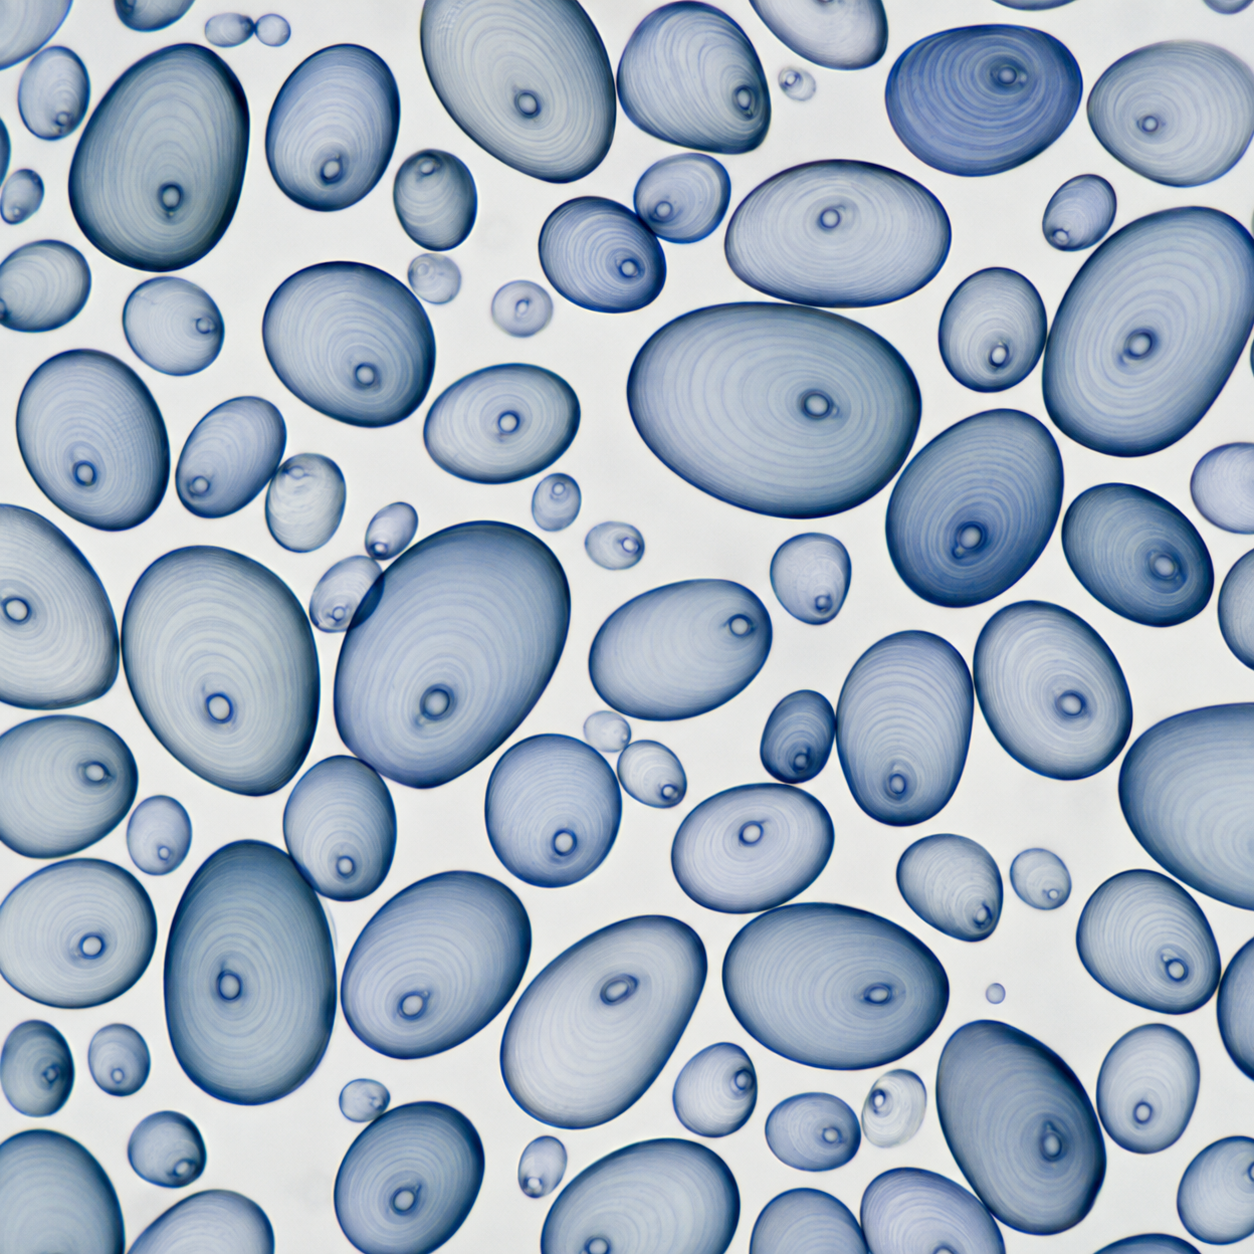
\includegraphics[width=0.96\linewidth]{images/book3/ai/b3-10-starch-grains.png}
\end{minipage}\hfill
\begin{minipage}[b]{0.52\linewidth}\centering
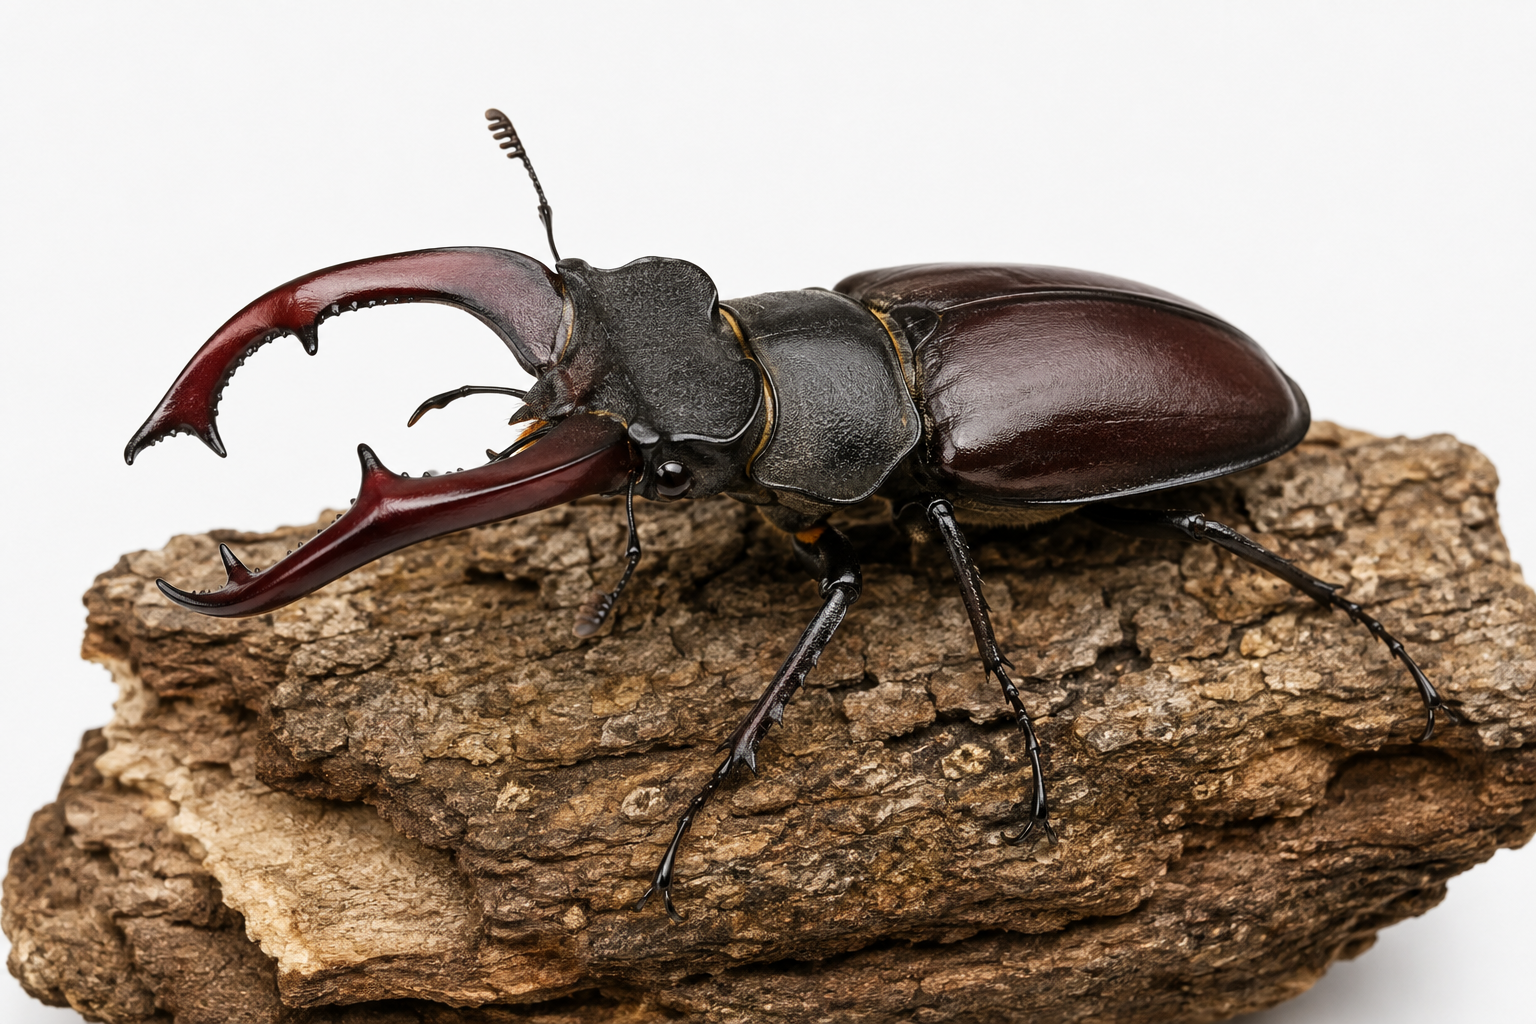
\includegraphics[width=0.96\linewidth]{images/book3/ai/b3-10-beetle-cuticle.png}
\end{minipage}

{\small À gauche~: grains d'\omterm{def:b1:carbohydrates:polysaccharide}{amidon} de pomme de terre au microscope,
colorés à l'eau iodée~; les anneaux concentriques sont les couches
d'amylopectine déposées jour après jour. À droite~: \omterm{def:b1:flowering-plant-organization:tissues}{cuticule} d'un
lucane --- des fibres de \omterm{def:b1:carbohydrates:polysaccharide}{chitine} dans une matrice protéique, durcies et
sombres~: la même architecture $\beta(1{\to}4)$ que la \omterm{def:b1:carbohydrates:polysaccharide}{cellulose}, sur un
autre sucre.}
\end{omfigure}

\begin{example}[Pourquoi le glycogène est ramifié]\label{ex:b1:carbohydrates:branching}
Le \omterm{def:b1:carbohydrates:polysaccharide}{glycogène} est dégradé depuis ses extrémités non réductrices, un
glucose à la fois, par la \omterm{def:b1:carbohydrates:polysaccharide}{glycogène} phosphorylase. Une chaîne non
ramifiée de \num{50000} glucoses aurait une seule extrémité de ce type
et libérerait un glucose par cycle d'enzyme~; une particule de \omterm{def:b1:carbohydrates:polysaccharide}{glycogène}
de même taille, ramifiée tous les douze résidus, en offre quelque
\num{2000} et en libère deux mille à la fois. La ramification garde
aussi la particule compacte et soluble. Les cent grammes de \omterm{def:b1:carbohydrates:polysaccharide}{glycogène} du
foie peuvent être mobilisés à dix grammes par heure~; le même glucose
stocké en une seule longue chaîne mettrait des années à se dérouler.
\end{example}

\begin{example}[Pourquoi ne pas stocker le glucose lui-même]\label{ex:b1:carbohydrates:osmotic}
Cent grammes de glucose (\qty{0.55}{mol}) dissous dans le \qty{1}{L}
d'eau des \omterm{def:b1:cell-unit-of-life:cell}{cellules} d'un foie ajouteraient \qty{0.55}{osmol/L} à un
\omterm{def:b1:eukaryotic-cell:organelle}{cytosol} à \qty{0.3}{osmol/L}~: les \omterm{def:b1:cell-unit-of-life:cell}{cellules} gonfleraient jusqu'à trois
fois leur volume et éclateraient. Sous forme de \omterm{def:b1:carbohydrates:polysaccharide}{glycogène}, le même
glucose fait $\num{7e18}$ particules, \qty{1e-5}{mol/L}, invisibles du
point de vue osmotique. Un polymère est une manière de stocker un très
grand nombre de molécules comme une seule.
\end{example}

\section{Glycoconjugués et paroi végétale}

\begin{definition}[Glycoprotéines, protéoglycanes, glycolipides]\label{def:b1:carbohydrates:glycoconjugate}
Des sucres sont fixés par covalence aux protéines et aux \omterm{def:b1:lipids:fattyacid}{lipides} pour
former des \emph{glycoconjugués}\index{glycoconjugue@glycoconjugué}. Une
\emph{glycoprotéine}\index{glycoproteine@glycoprotéine} porte de courtes chaînes
ramifiées (une douzaine de sucres) sur certains de ses résidus
d'asparagine, de sérine ou de thréonine, ajoutées dans le RE et le \omterm{def:b1:eukaryotic-cell:endomembrane}{Golgi}
(\cref{ch:b1:eukaryotic-cell})~: presque toute protéine sécrétée ou
membranaire en est une. Un \emph{protéoglycane}\index{proteoglycane@protéoglycane} est
un axe protéique portant de longues chaînes non ramifiées de
\omterm{def:b1:carbohydrates:glycosidic}{disaccharides} acides répétés, les
\emph{glycosaminoglycanes}\index{glycosaminoglycane} (hyaluronane,
chondroïtine-sulfate, héparine), qui fixent d'énormes quantités d'eau et
donnent au cartilage, au corps vitré et à la \omterm{def:b1:body-plans-tissues:connective}{matrice extracellulaire}
leur élasticité. Les \emph{glycolipides}\index{glycolipide} portent des
sucres sur une queue lipidique dans le feuillet externe de la membrane
plasmique. Avec les sucres des glycoprotéines, ils forment le
\emph{glycocalyx}\index{glycocalyx}, le manteau de sucres par lequel les
\omterm{def:b1:cell-unit-of-life:cell}{cellules} sont reconnues.
\end{definition}

\begin{example}[Les groupes sanguins]\label{ex:b1:carbohydrates:abo}
Les groupes sanguins ABO sont trois versions d'une même chaîne de sucres
portée par les \omterm{def:b1:carbohydrates:glycoconjugate}{glycolipides} et les \omterm{def:b1:carbohydrates:glycoconjugate}{glycoprotéines} de surface du globule
rouge~: la chaîne O se termine par un fucose~; A y ajoute une
N-acétylgalactosamine, B un galactose, par deux versions d'une même
enzyme~; les \omterm{def:b1:cell-unit-of-life:cell}{cellules} AB portent les deux. Un seul résidu de sucre
suffit au système immunitaire pour distinguer le soi de l'étranger, et à
une transfusion pour réussir ou pour tuer.
\end{example}

\begin{proposition}[La paroi de la cellule végétale]\label{prop:b1:carbohydrates:wall}
\index{paroi}
La paroi primaire d'une \omterm{def:b1:cell-unit-of-life:cell}{cellule} végétale est un composite renforcé de
fibres~: des microfibrilles de \omterm{def:b1:carbohydrates:polysaccharide}{cellulose} (le quart de la masse,
résistance à la traction) disposées en couches, reliées entre elles par
des \emph{hémicelluloses} (\omterm{def:b1:carbohydrates:polysaccharide}{polysaccharides} ramifiés qui se lient par
\omterm{def:b1:water-small-molecules:water}{liaisons hydrogène} aux microfibrilles et les pontent) et noyées dans un
gel de \emph{pectines} (\omterm{def:b1:carbohydrates:polysaccharide}{polysaccharides} acides qui retiennent l'eau et
le calcium et cimentent les \omterm{def:b1:cell-unit-of-life:cell}{cellules} entre elles dans la lamelle
moyenne), avec quelques pour cent de protéines. Elle est mince
(\qtyrange{0.1}{1}{\micro m}), perméable à l'eau et aux petits solutés,
et assez solide pour supporter \qty{1}{MPa} de \omterm{def:b1:eukaryotic-cell:plantcell}{turgescence}. Les \omterm{def:b1:cell-unit-of-life:cell}{cellules}
qui cessent de croître peuvent ajouter une épaisse \emph{paroi
secondaire}, plus riche en \omterm{def:b1:carbohydrates:polysaccharide}{cellulose} et pourvue de \emph{lignine},
polymère aromatique qui l'imperméabilise et la raidit~: le bois, ce sont
des parois secondaires.
\end{proposition}

\begin{omfigure}
\begin{tikzpicture}[font=\footnotesize, line cap=round]
  % matrix background
  \fill[omExo!8] (0,0) rectangle (8.4,3.6);
  % microfibrils: two layers of thick lines at different angles
  \foreach \y in {0.5,1.5,2.5,3.5} { \draw[line width=5pt, omDef!60] (0.2,\y-0.3) -- (8.2,\y-0.1); }
  \foreach \x in {1.2,3.2,5.2,7.2} { \draw[line width=5pt, omDef!35] (\x,0.1) -- (\x+0.6,3.5); }
  % hemicellulose tethers
  \foreach \x in {0.8,2.4,4.0,5.6,7.4} { \draw[thick, omProp] (\x,0.25) .. controls (\x+0.3,0.7) .. (\x+0.1,1.2) .. controls (\x-0.2,1.7) .. (\x+0.2,2.25) .. controls (\x+0.4,2.8) .. (\x,3.3); }
  % pectin gel dots
  \foreach \p in {(0.5,0.9),(1.9,2.9),(2.9,0.8),(4.6,2.1),(6.1,1.0),(6.9,3.1),(3.7,3.2),(7.9,1.9)} { \fill[omExo!70] \p circle (0.07); }
  % labels outside
  \node[anchor=west, align=left] at (8.7,3.0) {\textcolor{omDef!70!black}{microfibrilles de cellulose}\\ (résistance, en couches)};
  \node[anchor=west, align=left] at (8.7,1.8) {\textcolor{omProp!80!black}{hémicelluloses}\\ (pontent les fibrilles)};
  \node[anchor=west, align=left] at (8.7,0.6) {\textcolor{omExo!70!black}{gel de pectines}\\ (matrice hydratée, ciment)};
\end{tikzpicture}

{\small La paroi primaire d'une \omterm{def:b1:cell-unit-of-life:cell}{cellule} végétale comme composite~: des
couches de microfibrilles de \omterm{def:b1:carbohydrates:polysaccharide}{cellulose} (bleu) reliées par des chaînes
d'hémicelluloses (orange) dans un gel de pectines (vert). Des fibres
rigides dans une matrice humide~: le principe de la fibre de verre,
inventé un milliard d'années plus tôt.}
\end{omfigure}

\section{Les sucres comme carburant et comme carbone}

\begin{proposition}[La place du glucose]\label{prop:b1:carbohydrates:fuel}
Les \omterm{def:b1:carbohydrates:monosaccharide}{glucides} rendent \qty{17}{kJ/g} à l'oxydation et sont le carburant
que toute \omterm{def:b1:cell-unit-of-life:cell}{cellule} sait employer, avec ou sans oxygène
(\cref{ch:b1:respiration-fermentation})~; le glucose est le sucre du
sang (\qty{5}{mmol/L}), le saccharose celui de la sève, et l'\omterm{def:b1:carbohydrates:polysaccharide}{amidon} et
le \omterm{def:b1:carbohydrates:polysaccharide}{glycogène} leurs réserves. Les sucres sont aussi le carbone à partir
duquel la \omterm{def:b1:cell-unit-of-life:cell}{cellule} fabrique tout le reste~: les pentoses des nucléotides,
le glycérol des \omterm{def:b1:lipids:fattyacid}{lipides}, les squelettes carbonés des acides aminés
quittent tous les voies des sucres
(\cref{ch:b1:biosyntheses-integration}). La photosynthèse fabrique
d'abord du sucre~; le reste suit.
\end{proposition}

\begin{example}[Le sucre d'une journée]\label{ex:b1:carbohydrates:day}
Un humain mange quelque \qty{300}{g} de \omterm{def:b1:carbohydrates:monosaccharide}{glucides} par jour, presque tous
sous forme d'\omterm{def:b1:carbohydrates:polysaccharide}{amidon} et de saccharose~; l'intestin les \omterm{prop:b1:water-small-molecules:families}{hydrolyse} en
glucose, fructose et galactose, le foie convertit les deux derniers en
glucose, et le glucose circule à raison de \qty{5}{g} dans tout le sang
--- vingt minutes de réserve pour l'encéphale, qui en consomme
\qty{120}{g} par jour, renouvelées en continu à partir du \omterm{def:b1:carbohydrates:polysaccharide}{glycogène} du
foie. Le cristallin, les globules rouges et la médulla rénale vivent du
seul glucose~; rien d'autre dans l'alimentation ne peut le remplacer, et
quand il vient à manquer le foie en fabrique à partir des protéines.
\end{example}

\section{Exercices}

\begin{exercise}[$\star$]\label{exo:b1:carbohydrates:1}
Classer le glucose, le fructose, le ribose et le glycéraldéhyde par
nombre de carbones et selon qu'il s'agit d'un \omterm{def:b1:carbohydrates:monosaccharide}{aldose} ou d'un \omterm{def:b1:carbohydrates:monosaccharide}{cétose}.
\end{exercise}

\begin{exercise}[$\star$]\label{exo:b1:carbohydrates:2}
Qu'est-ce qu'un carbone anomérique, et pourquoi un \omterm{def:b1:carbohydrates:glycosidic}{disaccharide} dont les
deux carbones anomériques sont engagés dans la liaison ne réagit-il pas
avec la liqueur de Benedict~?
\end{exercise}

\begin{exercise}[$\star$]\label{exo:b1:carbohydrates:3}
Nommer les monomères et les liaisons de l'\omterm{def:b1:carbohydrates:polysaccharide}{amidon}, du \omterm{def:b1:carbohydrates:polysaccharide}{glycogène}, de la
\omterm{def:b1:carbohydrates:polysaccharide}{cellulose} et de la \omterm{def:b1:carbohydrates:polysaccharide}{chitine}.
\end{exercise}

\begin{exercise}[$\star$]\label{exo:b1:carbohydrates:4}
D'après la figure de Haworth, indiquer la position (haut ou bas) des
hydroxyles portés par les carbones 1 à 4 de l'$\alpha$-D-glucose, puis
dessiner ou décrire l'$\alpha$-D-galactose.
\end{exercise}

\begin{exercise}[$\star\star$]\label{exo:b1:carbohydrates:5}
Expliquer, à partir de la géométrie des liaisons $\alpha$ et $\beta$,
pourquoi l'amylose forme une hélice et la \omterm{def:b1:carbohydrates:polysaccharide}{cellulose} un ruban, et
pourquoi le test à l'eau iodée fonctionne sur la première et non sur la
seconde.
\end{exercise}

\begin{exercise}[$\star\star$]\label{exo:b1:carbohydrates:6}
Trois tubes contiennent du glucose, du saccharose et de l'\omterm{def:b1:carbohydrates:polysaccharide}{amidon}.
Concevoir une suite de tests (Benedict, eau iodée, \omterm{prop:b1:water-small-molecules:families}{hydrolyse} acide) qui
identifie chacun, en donnant le résultat attendu de chaque test.
\end{exercise}

\begin{exercise}[$\star\star$]\label{exo:b1:carbohydrates:7}
Une particule de \omterm{def:b1:carbohydrates:polysaccharide}{glycogène} contient \num{50000} résidus de glucose,
ramifiés tous les 12. Estimer le nombre d'extrémités non réductrices et
le comparer à celui d'une molécule d'amylose de même taille. Si la
phosphorylase libère un glucose par seconde à chaque extrémité, combien
de temps chacune met-elle à libérer \qty{10}{\%} de son glucose~?
\end{exercise}

\begin{exercise}[$\star\star$]\label{exo:b1:carbohydrates:8}
Les microfibrilles de \omterm{def:b1:carbohydrates:polysaccharide}{cellulose} ont une résistance à la traction
d'environ \qty{1}{GPa}. Une \omterm{def:b1:cell-unit-of-life:cell}{cellule} de \qty{50}{\micro m} de diamètre à
paroi de \qty{0.5}{\micro m} d'épaisseur supporte une \omterm{def:b1:eukaryotic-cell:plantcell}{turgescence} de
\qty{0.8}{MPa}. Calculer la contrainte dans la paroi ($\sigma = Pr/2t$
pour une sphère) et la comparer à la résistance.
\end{exercise}

\begin{exercise}[$\star\star$]\label{exo:b1:carbohydrates:9}
Intolérance au lactose~: les adultes dépourvus de lactase intestinale
souffrent de crampes et de diarrhée après avoir bu du lait. Expliquer,
à l'aide de la liaison que rompt la lactase, ce qu'il advient du lactose
non digéré dans le côlon (bactéries, \omterm{def:b1:membranes-transport:osmosis}{osmose}).
\end{exercise}

\begin{exercise}[$\star\star\star$]\label{exo:b1:carbohydrates:10}
Une vache mange \qty{10}{kg} de matière sèche d'herbe par jour, dont
\qty{40}{\%} de \omterm{def:b1:carbohydrates:polysaccharide}{cellulose}. Elle n'a pas de cellulase. Expliquer comment
elle tire pourtant de l'énergie de la \omterm{def:b1:carbohydrates:polysaccharide}{cellulose}, pourquoi le processus
doit se dérouler avant l'intestin grêle, et estimer l'énergie en jeu si
\qty{60}{\%} de la \omterm{def:b1:carbohydrates:polysaccharide}{cellulose} est fermentée et rend \qty{12}{kJ} de
produits utilisables par gramme.
\end{exercise}

\begin{exercise}[$\star\star\star$]\label{exo:b1:carbohydrates:11}
Les antigènes des groupes A et B diffèrent par un sucre ajouté par deux
versions d'une transférase~; le groupe O n'en a aucun. Expliquer
pourquoi une personne O peut donner ses globules rouges à tout le monde
mais n'en recevoir que d'un O, et ce que doit contenir le \omterm{def:b1:mammal-organization:compartments}{plasma} d'une
personne A.
\end{exercise}

\begin{exercise}[$\star\star\star$]\label{exo:b1:carbohydrates:12}
«~Le glucose est le carburant universel, la \omterm{def:b1:carbohydrates:polysaccharide}{cellulose} le matériau de
construction universel, et ce sont la même molécule.~» Discuter en un
paragraphe~: ce que la phrase dit de juste, ce qu'une seule liaison
change, et ce que cela dit du rapport entre chimie et biologie.
\end{exercise}

\section{Problème~: l'arbre du glycogène}

\begin{problem}[{Problème du week-end --- une particule de glycogène
comptée branche par branche, la réserve du foie pesée et sa libération
chronométrée, le prix osmotique que la polymérisation évite, jusqu'au
débit de libération de glucose du foie}]
\label{pb:b1:carbohydrates:1}
Une particule de \omterm{def:b1:carbohydrates:polysaccharide}{glycogène} est un arbre de chaînes~: une chaîne interne
de \qty{13}{} résidus de glucose porte deux branches, chacune de
\qty{13}{} résidus et portant à son tour deux branches, et ainsi de
suite sur \qty{12}{} rangs~; les chaînes du rang le plus externe ne sont
pas ramifiées. Chaque résidu de glucose du polymère a une masse de
\qty{162}{g/mol}. Un foie humain au repos, de \qty{1.5}{kg}, contient
\qty{100}{g} de \omterm{def:b1:carbohydrates:polysaccharide}{glycogène} dans \qty{1.0}{L} d'eau cellulaire, et libère
du glucose dans le sang à \qty{10}{g/h} entre les repas. La \omterm{def:b1:carbohydrates:polysaccharide}{glycogène}
phosphorylase retire un glucose d'une extrémité non réductrice par
cycle, à raison de \qty{20}{} cycles par seconde et par molécule
d'enzyme.

\medskip
\noindent\textbf{Partie I --- Compter l'arbre.}
\begin{enumerate}
  \item Combien de chaînes le rang $t$ contient-il ($t = 1$ pour la
        chaîne interne)~? Donner le nombre pour les rangs 1, 2, 3 et 12.
  \item Calculer le nombre total de chaînes de la particule.
  \item Calculer le nombre total de résidus de glucose.
  \item Calculer la masse de la particule, en daltons et en grammes.
  \item Quelle fraction de toutes les chaînes se trouve au rang le plus
        externe~? Combien d'extrémités non réductrices la particule
        offre-t-elle~?
  \item Combien d'extrémités non réductrices possède une molécule
        d'amylose comptant le même nombre de résidus~?
  \item Si chaque rang ajoute \qty{1.9}{nm} au rayon, calculer le
        diamètre de la particule et le comparer à celui d'un ribosome
        (\qty{25}{nm}).
\end{enumerate}

\medskip
\noindent\textbf{Partie II --- La réserve du foie.}
\begin{enumerate}[resume]
  \item Calculer le nombre de particules du foie.
  \item Calculer le glucose que représente la réserve, en moles et en
        grammes de glucose libre (\qty{180}{g/mol}).
  \item Le \omterm{def:b1:carbohydrates:polysaccharide}{glycogène} fixe \qty{3}{g} d'eau par gramme. Quelle masse du
        foie le \omterm{def:b1:carbohydrates:polysaccharide}{glycogène} et son eau représentent-ils~?
  \item Calculer le débit de libération de \qty{10}{g/h} en molécules de
        glucose par seconde.
  \item Combien d'heures la réserve dure-t-elle à ce débit~? À la
        demande de quel \omterm{def:b1:mammal-organization:organ}{organe} cette libération répond-elle
        principalement~?
\end{enumerate}

\medskip
\noindent\textbf{Partie III --- Extrémités et enzymes.}
\begin{enumerate}[resume]
  \item Calculer le nombre total d'extrémités non réductrices du foie.
  \item Si toutes les extrémités étaient attaquées à la fois à
        \qty{20}{} glucoses par seconde, quel serait le débit de
        libération, en grammes par seconde~? Le comparer au débit réel.
  \item Combien de molécules de phosphorylase, travaillant chacune à
        \qty{20}{} par seconde, sont nécessaires pour le débit réel~?
  \item Supposons les mêmes \qty{100}{g} stockés en chaînes d'amylose de
        la même taille que les particules. Calculer le nombre
        d'extrémités et le débit de libération maximal.
  \item Expliquer pourquoi les points de branchement sont la clé de la
        réponse du foie à une baisse de la glycémie en quelques minutes.
\end{enumerate}

\medskip
\noindent\textbf{Partie IV --- Le prix osmotique.}
\begin{enumerate}[resume]
  \item Si les \qty{100}{g} étaient dissous en glucose libre dans le
        \qty{1.0}{L} d'eau cellulaire, quelle osmolarité cela
        ajouterait-il~?
  \item Comparer avec les \qty{0.3}{osmol/L} du \omterm{def:b1:eukaryotic-cell:organelle}{cytosol} et prédire ce
        qu'il adviendrait des \omterm{def:b1:cell-unit-of-life:cell}{cellules}.
  \item Calculer l'osmolarité due aux particules de \omterm{def:b1:carbohydrates:polysaccharide}{glycogène}
        elles-mêmes.
  \item Calculer le \omterm{def:b1:membranes-transport:osmosis}{potentiel hydrique} que créerait le glucose libre
        ($\Psi_s = -RTc$, $RT = \qty{2.58}{MPa.L/mol}$) et la pression
        qu'une paroi de type végétal devrait supporter.
  \item Le muscle stocke \qty{400}{g} de \omterm{def:b1:carbohydrates:polysaccharide}{glycogène} dans \qty{30}{kg} de
        muscle mais ne peut pas libérer de glucose dans le sang.
        Proposer une raison, compte tenu de ce à quoi sert le \omterm{def:b1:carbohydrates:polysaccharide}{glycogène}
        dans un muscle.
  \item Une pomme de terre stocke l'\omterm{def:b1:carbohydrates:polysaccharide}{amidon} en grains de
        \qty{50}{\micro m}, et non en particules de \omterm{def:b1:carbohydrates:polysaccharide}{glycogène} de
        \qty{40}{nm}. Rattacher cette différence à l'échelle de temps de
        mobilisation dont chaque \omterm{def:b1:organism-environment:organism}{organisme} a besoin.
  \item Après un repas, le foie reconstitue \qty{100}{g} de \omterm{def:b1:carbohydrates:polysaccharide}{glycogène} en
        quatre heures. Calculer le débit en résidus de glucose par
        seconde et le coût en \omterm{def:b1:water-small-molecules:atp}{ATP} si l'ajout d'un résidu coûte deux
        équivalents \omterm{def:b1:water-small-molecules:atp}{ATP}.
  \item Énoncer le résultat~: le débit de libération de glucose du foie
        en molécules par seconde, le nombre d'extrémités non réductrices
        qui le rend possible, et l'osmolarité que le polymère épargne
        aux \omterm{def:b1:cell-unit-of-life:cell}{cellules}.
\end{enumerate}
\end{problem}
